\part{Fyzikální model}

\section{Model kamene}
Broušený kámen je modelován jako konvexní mnohostěn \cite{Pohl2002}. Brusné kotouče považujeme za dokonale rovinné. Uchycení kamene při broušení zjednodušíme na absolutně tuhé bez známek pružnosti či ohybu. Fasety potom můžeme modelovat jako rovinné plochy. Orientace a umístění fasety získáme z výkresu nebo předchozího měření. 

Přechody mezi fasetami jsou v ideálním případě ostré hrany. Z důvodu abraze hran v procesu výroby kamene jsou hrany obroušeny do přibližně oblého tvaru. K přiblížení modelu reálnému obroušení hran aproximujeme hranu množstvím rovinných faset se vzájemnou polohou odpovídající poloměru křivosti hrany.  
  
\begin{figure}[htps]
\centering
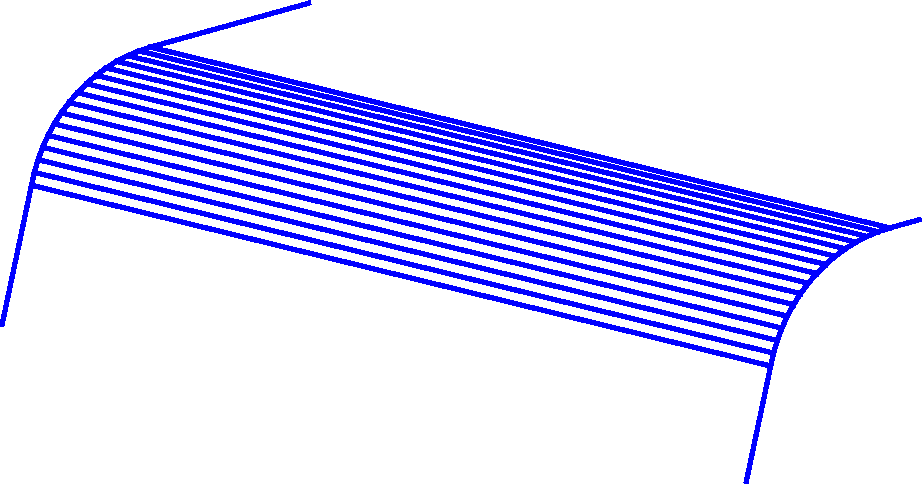
\includegraphics[width=0.5\linewidth]{edge_ex.pdf}
\caption{Detail aproximace přechodu mezi fasetami.}
\label{fig: edge}
\end{figure}  

\section{Model svazku}
Svazek světla v LADOKU reprezentuje nerozbíhající se konvexní hranol. Vlivem odrazu a lomu se konvexní tvar zachová. Fasety jsou také konvexní, proto se konvexita zachová i při štěpení svazku. Po opuštění kamene jsou svazky definovány zářivým tokem, plochou a směrem, které lze vyjádřit pomocí azimutu a elevace. Stokesovy koeficienty definují polarizaci svazku \cite{bodlakLADOK}. 

Zaznamenána je celá cesta svazku. V každém bodě trasy známe směr a tvar svazku vyjádřený pomocí polygonu. 

Model nepostihuje situace, při kterých dochází k rozbíhavosti světla.
\begin{itemize}
\item Pokud jsou v materiálu přítomné nečistoty, praskliny, vzduchové bubliny apod., světelný svazek se rozptýlí.
\item Rozptyl světelných svazků vzniká také vlivem nedokonalého vyleštění faset, a to jak při lomu tak při odrazu.
\item Přítomnost hran v kameni způsobí ohyb světla (difrakci) \cite{HandbookDiff}.
\end{itemize}


\paragraph{Ocásky}
\hspace{1mm}

V ideálním případě lze ve snímaném obraze pozorovat pouze dopady světelných svazků, které vznikly kombinací odrazů a lomů zdrojového svazku od faset broušeného kamene. U~reálného kamene ovšem v obraze pozorujeme tenké slábnoucí přímky vycházející ze stopy světelného svazku, ocásky. Tyto ocásky vznikají díky lomu/odrazu světelného svazku od neostrých hran broušeného kamene.

\begin{figure}[h!]
\begin{center}
\scalebox{.9}{ \input{xfig/tails.pstex_t}}
\end{center}
\caption[Příklad snímaného obrazu s vyznačením obrazů svazků a ocásků.]{Příklad snímaného obrazu s vyznačením obrazů svazků a ocásků.}
\label{fig:tail_ex1}
\end{figure}


Vnik ocásků si ukážeme při lomu světla na oblé hraně kamene. Situaci budeme uvažovat v 2D prostoru, kde platí obecně stejné principy jako ve 3D. Světlo nahradíme paprsky světla se směrem šíření $\vec{v_i}$. 

Zvolíme dvě fasety svírající úhel \SI{45}{\degree}. Přechod mezi fasetami aproximujeme. Vznikne posloupnost úseček, které propojují fasety. Každé úsečce přiřadíme normálový vektor $\vec{n}$.  

\begin{figure}[h!]
\centering
\begin{minipage}[c]{0.43\textwidth}
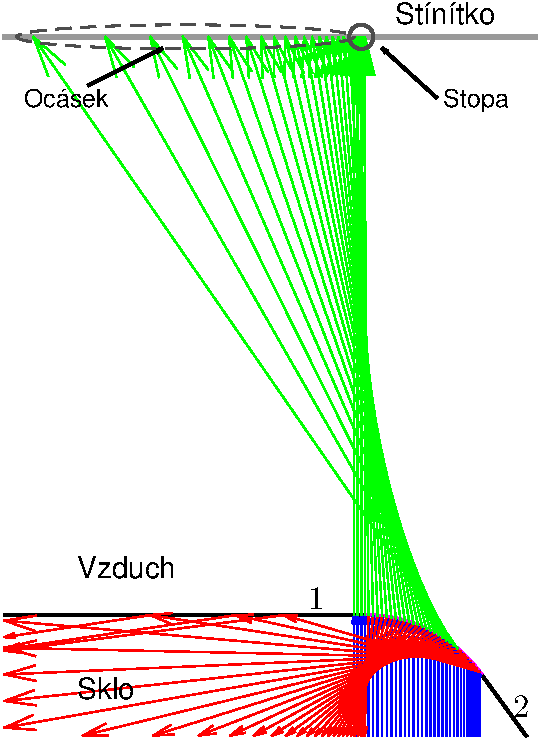
\includegraphics[height=9cm]{edgeOutFar.pdf}
\end{minipage}
\begin{minipage}[c]{0.53\textwidth}
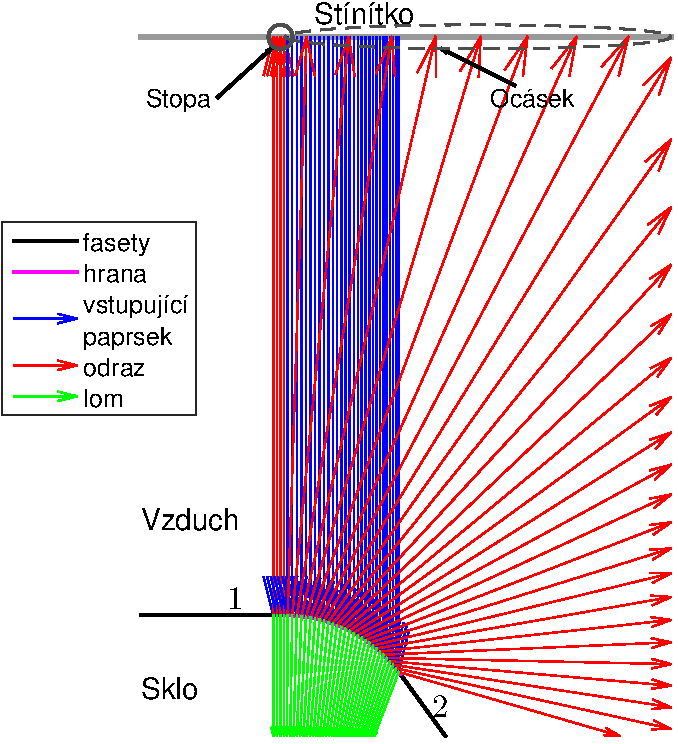
\includegraphics[height=9cm]{edgeInFar.pdf}
\end{minipage}

\caption[Vznik ocásků.]{Vznik ocásků na stínítku při dopadu světelných paprsků na hranu mezi fasetami \textbf{1} a \textbf{2}. Vpravo: paprsky se lomí ze skla do kamene. Vlevo: paprsky se lomí ze vzduchu do skla. Situace pro index lomu vzduchu $n_a = 1$ a index lomu skla $n_g = 1.5$.}
\label{fig:edgeIn}
\end{figure}
Aplikací Snellova zákonu a zákonu odrazu na $\vec{n}$ a $\vec{v_i}$ vypočítáme směr lomu a odrazu světelných paprsků.

Z Fresnelových rovnic \cite{Handbook} víme, že dochází nejen k lomu světla, ale část světla se odrazí. Poměr intenzity odraženého a lomeného světla závisí na polarizaci světla a dopadajícím úhlu. V této ukázce uvažujeme nepolarizované světlo. 

Na obr. \ref{fig:edgeIn} dopadají paprsky světla ze vzduchu na sklo i ze skla do vzduchu. V obou případech se odražené i lomené paprsky projeví  na stínítku jako ocásky.

Pokusíme se prozkoumat jak se mění intenzita ocásku v závislosti na úhlu $\beta$. Úhel $\beta$ uvádí absolutní úhlovou odchylku směru odraženého resp. lomeného svazku na hraně od směru odraženého resp. lomeného svazku přes fasetu \textbf{1}.  

Pro úhel $\beta$ určíme poměr intenzity ocásku $I_{\beta}$ a intenzity dopadajícího paprsku $I_0$. 
\begin{equation}
 \frac{I_\beta}{I_0}  = \frac{\rho_{{max}}}{\rho_\beta}\cdot R_\beta
\end{equation}
pro odražené paprsky a 
\begin{equation}
 \frac{I_\beta}{I_0}  = \frac{\rho_{max}}{\rho_\beta}\cdot (1-R_\beta)
\end{equation}
pro lomené paprsky, kde  

	\begin{tabular}{l l}
	$\rho_{\beta}$  & 	- hustota paprsků pro daný úhel $\beta\,$,\\
	$\rho_{{max}}$ 	&	- maximální hustota paprsků,\\
	$R_\beta$		&	- odrazivost z Fresnelových rovnic \cite{Handbook}.	 \\
	
	\end{tabular}
	\vspace{1mm}

\begin{figure}[h!]
\centering
\begin{minipage}[c]{0.48\textwidth}
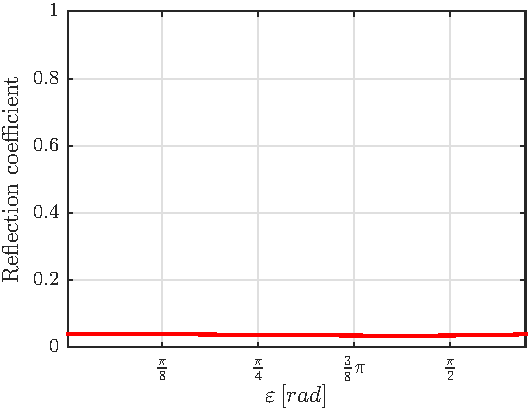
\includegraphics[width=\textwidth]{edgeIn_reflection.pdf}
\end{minipage}
\begin{minipage}[c]{0.48\textwidth}
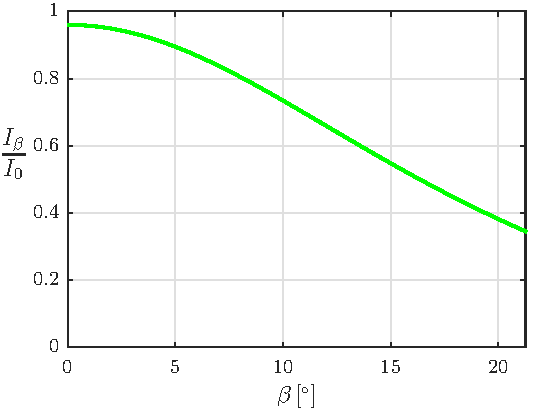
\includegraphics[width=\textwidth]{edgeIn_refraction.pdf}
\end{minipage}
\caption[Poměrná velikost intenzity ocásku případ lomu ze vzduchu do skla.]{Poměrná velikost intenzity ocásků v závislosti na úhlu $\beta$ pro případ lomu ze vzduchu do skla. Vpravo: odraz. Vlevo: lom.}
\label{fig:edgeInGraf}
\end{figure}

\begin{figure}[h!]
\centering
\begin{minipage}[c]{0.48\textwidth}
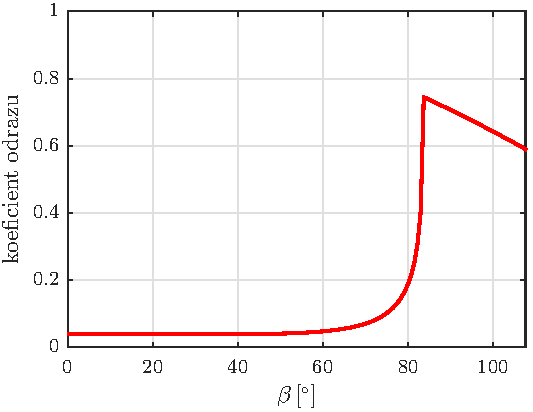
\includegraphics[width=\textwidth]{edgeOut_reflection.pdf}
\end{minipage}
\begin{minipage}[c]{0.48\textwidth}
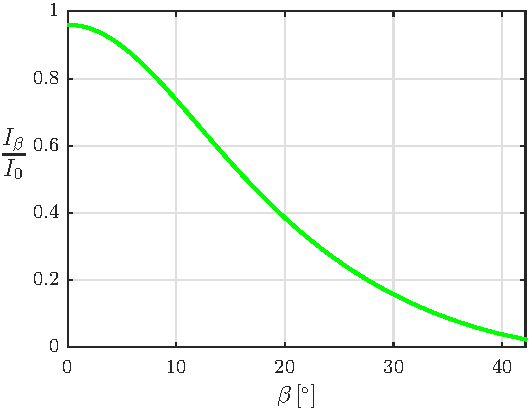
\includegraphics[width=\textwidth]{edgeOut_refraction.pdf}
\end{minipage}
\caption[Poměrná velikost intenzity ocásku případ lomu ze skla do vzduchu.]{Poměrná velikost intenzity ocásků v závislosti na úhlu $\beta$ pro případ lomu ze skla do vzduchu. Vpravo: odraz. Vlevo: lom.}
\label{fig:edgeOutGraf}
\end{figure}

Z grafů \ref{fig:edgeInGraf} a \ref{fig:edgeOutGraf} je patrné, že ocásky budeme pozorovat různě dlouhé a z vysokou variabilitou z hlediska intenzity. 
	  
 Intenzita a délka ocásku je ovlivněna i dalšími faktory, jako je např. délka a ostrost hrany. Všechny faktory, které ovlivňují intenzitu ocásku prozatím nejsme schopni v programu LADOK zahrnout do matematického modelu, proto pro prování svazků bude užitečná především informace o směru ocásku. 
 
 \newpage
 \paragraph{Třídy svazků}
 \hspace{1mm}
 
 Svazky jsou definovány podle posloupnosti dopadových faset. Tento způsob popisu při opakovaném použití není přehledný.
 Pro lepší orientaci svazky rozdělíme do tříd a budeme pracovat pouze s názvem třídy. Rozdělení do tříd je v příloze ....  


\section{Model stínítka}
\label{sec:stinitko}
Po dopadu laserového svazku na stínítko se záření difuzně odrazí. Odrazivé vlastnosti materiálu závisí na úhlu odpadajícího světla a lze je matematicky popsat pomocí modelu zvaného BRDF (Bidirectional reflectance distribution function). Část rozptýleného světla dopadne na stínítko do okolí ostatních stop. 

%%tohle bych zařadil na později
%Laserové stopy chceme detekovat v černobílém HDR snímku půlkulového stínítka, na které dopadá část laserových svazků vystupujících z nasvíceného kamene. Snímek ze zatížen radiálním zkreslením, které je způsobeno vlastností optické soustavy objektivu. Radiální zkreslení bylo určeno v předchozí bakalářské práci \cite{Drapela}. Snímek lze pomocí transformace z \cite{Drapela} zkreslení zbavit. Z \cite{Drapela} navíc známe transformaci mezi pozicí bodu v nezkresleného snímku a odpovídajícím parametrům azimutu a elevace.


\section{Model kamery}
\label{sec:poisson}
 Použitý CCD snímač má $2050^2$ pixelů. Každému pixelu odpovídá jeden samostatný snímač, který funguje na principu počítání přicházejících fotonů po dobu expozice. Počet přicházejících fotonů v daném časovém intervalu se řídí Poissonovým rozdělením. Pravděpodobnost, že napočítáme $n$ fotonů je 
 
 \begin{equation}
    P(\mathrm{X} = n)=\frac{\lambda ^{n}\,\mathrm{e}^{-\lambda}}{n!}\,,
 \end{equation}
 kde $\lambda$ je střední hodnota a $\mathrm{X}$ náhodná veličina, která popisuje dopad fotonů na snímač. 

\clearpage







